\documentclass[tikz,border=10pt]{standalone}
\usepackage{tikz}
\usetikzlibrary{shapes.geometric, arrows.meta, positioning}

% Define styles
\tikzstyle{process} = [rectangle, minimum width=3cm, minimum height=1cm, text centered, draw=black, fill=white, text width=3cm]
\tikzstyle{decision} = [diamond, minimum width=2cm, minimum height=1cm, text centered, draw=black, fill=gray!20, aspect=2]
\tikzstyle{endpoint} = [rectangle, minimum width=2.5cm, minimum height=1cm, text centered, draw=black, fill=white]
\tikzstyle{block} = [rectangle, minimum width=2.5cm, minimum height=1cm, text centered, draw=red, fill=white, text=red, line width=1pt]
\tikzstyle{consensus} = [rectangle, minimum width=2.5cm, minimum height=1cm, text centered, draw=green!60!black, fill=white, text=green!60!black, line width=1pt]
\tikzstyle{arrow} = [thick,->,>=Stealth]

\begin{document}
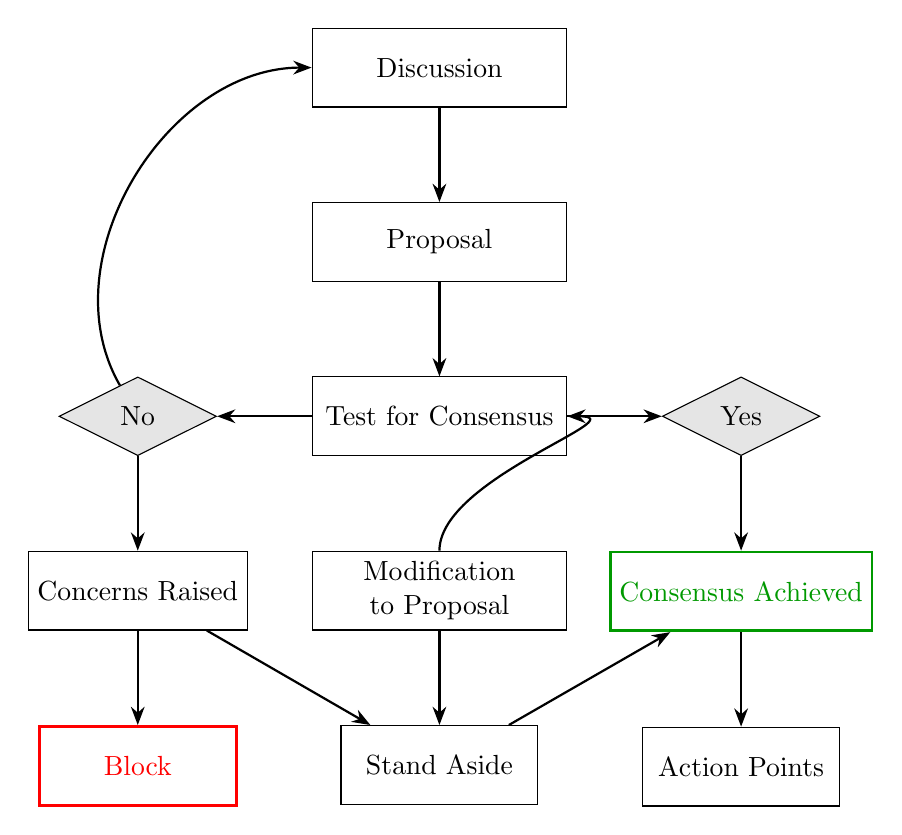
\begin{tikzpicture}[node distance=1.5cm]

% Nodes
\node (discussion) [process] {Discussion};
\node (proposal) [process, below=1.2cm of discussion] {Proposal};
\node (test) [process, below=1.2cm of proposal] {Test for Consensus};
\node (yes) [decision, right=1.2cm of test] {Yes};
\node (no) [decision, left=1.2cm of test] {No};
\node (modification) [process, below=1.2cm of test] {Modification to Proposal};
\node (concerns) [endpoint, below=1.2cm of no] {Concerns Raised};
\node (standAside) [endpoint, below=1.2cm of modification] {Stand Aside};
\node (consensusAchieved) [consensus, below=1.2cm of yes] {Consensus Achieved};
\node (blockNode) [block, below=1.2cm of concerns] {Block};
\node (actionPoints) [endpoint, below=1.2cm of consensusAchieved] {Action Points};

% Arrows
\draw [arrow] (discussion) -- (proposal);
\draw [arrow] (proposal) -- (test);
\draw [arrow] (test) -- (yes);
\draw [arrow] (test) -- (no);
\draw [arrow] (yes) -- (consensusAchieved);
\draw [arrow] (no) -- (concerns);
\draw [arrow] (modification) -- (standAside);
\draw [arrow] (concerns) -- (blockNode);
\draw [arrow] (consensusAchieved) -- (actionPoints);
\draw [arrow] (concerns) -- (standAside);
\draw [arrow] (standAside) -- (consensusAchieved);

% Curved arrows
\draw [arrow] (no) to[out=120, in=180] (discussion);
\draw [arrow] (modification) to[out=90, in=0] (test);

\end{tikzpicture}
\end{document}
